\glava{Идентификация параметров модели}

Для построения математической модели используются макроэкономические показатели статистического агенства ООН \cite{unstat}.

Расчеты могут быть выполнены:
\begin{itemize}
	\item В долларах \nom{США}{Соединенные Штаты Америки}.
	\item В национальной валюте.
\end{itemize}

Также существует два вида цен:
\begin{itemize}
	\item \textbf{Текущие.}
	Цены на какую-либо конкретную дату, например на 1 апреля, либо средние за год цены.
	\item \textbf{Постоянные.}
	Цены определенного периода, принимаемые за основу расчета макроэкономических показателей.
	Эти цены не учитывают уровень инфляции.
	На момент написания работы этот период --- 2015 год.
\end{itemize}
Если периоды текущих и постоянных цен совпадают, то и цены тоже соответственно совпадают.

Введем специальные обозначения, которые представлены в таблице \ref{desig_of_params}.

\begin{table}[]
	\centering
	\begin{tabular}{|c|c|}
	\hline
	\multicolumn{1}{|c|}{Параметр} & \multicolumn{1}{c|}{Описание} \\ \hline
	$t$                          &Значение, получаемое при вычитании 2010 из текущего года\\
	$Y$                          & ВВП                                                   \\
	$I$                          & импорт                                                \\
	$J$                          & размер инвестиций                                     \\
	$C$                          & общие расходы на потребление                          \\
	$E$                          & экспорт                                               \\ \hline
\end{tabular}
\caption{Специальные обозначения для параметров}\label{desig_of_params}
\end{table}

Все переменные с нижним индексом $_{stat}$ обозначают статистические данные.
В противном случае, это параметры модели.
Переменные с нижним индексом $_{const}$ обозначают постоянные цены.
В противном случае текущие.

Таблицы найденных статистических данных для Республики Сербия  представлены в приложении \ref{first_app}.
Все найденные показатели представлены в текущих и постоянных ценах.
Все данные представлены с 1993 года, так как это был переломный момент в истории страны.

Первым делом посчитаем индексы цен, определим поведение цен в среднем.
Индекс цен представляет собой соотношение макроэкономических показателей данного периода в текущих и постоянных ценах.
Для этого воспользуемся формулой:
\begin{equation}
	P(X(t)) = \cfrac{X(t)}{X_{const}(t)}
\end{equation}
где $X(t)$ это макроэкономический показатель.

На Рис. \ref{fig:index_rsd} и Рис. \ref{fig:index_usd} видна динамика поведения цен.
\begin{figure}
	\centering
	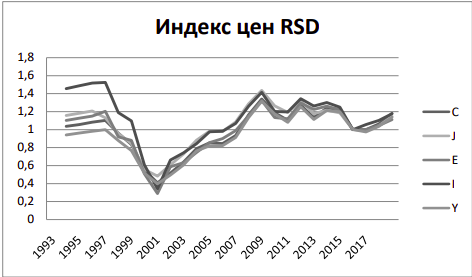
\includegraphics[scale=0.8]{images/index_rsd.png}
	\caption{Индекс цен RSD 1993 -- 2018}
	\label{fig:index_rsd}
\end{figure}
\begin{figure}
	\centering
	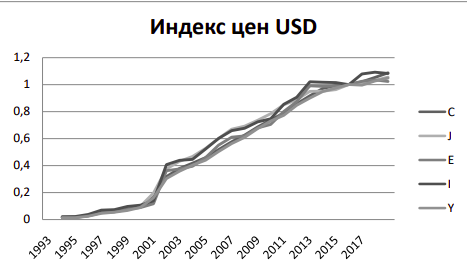
\includegraphics[scale=0.8]{images/index_usd.png}
	\caption{Индекс цен USD 1993 -- 2018}
	\label{fig:index_usd}
\end{figure}

В дальнейшем все расчеты будут проведены в постоянных ценах национальной валюты 2015 года.
